\documentclass[titlepage,12pt]{article}
\usepackage[utf8]{inputenc}
\usepackage{graphicx}
\usepackage{glossaries}
\usepackage{amsmath}
\usepackage{fullpage}
\usepackage{tocbibind}
\usepackage{siunitx}
\usepackage{url}


\title{\num{1e-30} \textmd{Seconds}}
\author{\textbf{K Scott Perrin}}
\date{October 2017}
\begin{document}

\maketitle


\pagebreak

%%%%%%%%%%%%%%%%%%%%%%%%%%%%%%%%%%%%%%%%%%%%%%%%%%%%%%%%%%%%%%%%%%%%%%%%
% Auto-generated table of contents, list of figures and list of tables %
%%%%%%%%%%%%%%%%%%%%%%%%%%%%%%%%%%%%%%%%%%%%%%%%%%%%%%%%%%%%%%%%%%%%%%%%

\begin{abstract}
\begin{center}
Cosmology glossary and bibliography. This paper was written using LaTeX.
\end{center}
\end{abstract}

\pagebreak
\tableofcontents
\pagebreak

\section{Timeline}

\begin{table}[htbp]
\begin{center}
\begin{tabular}{|c|c|c|c|} \hline
\textbf{Event/Epoch} & \textbf{Redshift}$z$ & \textbf{Time} & \textbf{Temp, K} \\ \hline
Big bang & $\infty$ & 0 & $\infty$\\ \hline
TOE/Planck time & $\cdots$ & $10^{-43}$ sec & $10^{32}$\\ \hline
GUT/Strong force separates from Weak/EM & $\cdots$ & $10^{-36}$ sec & $10^{28}$\\ \hline
Inflation starts & $\cdots$ & $10^{-36}$ sec & $10^{28}$\\ \hline
Inflation ends & $\cdots$ & $10^{-34}$ sec & $10^{28}$\\ \hline
Weak force separates from EM & $\cdots$ & $10^{-12}$ sec & $10^{16}$\\ \hline
Radiation-nucleon soup & $\cdots$ & $10^{-1}$ sec & $3\cdot 10^{10}$\\ \hline
Neutrinos decouple from nucleons & $\cdots$ & $1$ sec & $3\cdot 10^{9}$\\ \hline
Big bang Nucleosynthesis begins & $\cdots$ & $200$ sec & $8\cdot 10^{8}$\\ \hline
BBN ends = H, He, Li nuclei & $\cdots$ & $15$ min & $3\cdot 10^{8}$\\ \hline
Radiation-matter energy density equality & 3570 & $~50,000$ yrs & 9,390\\ \hline
Recombination (ionized plasma to neutral atoms) & 1380 & $~250,000$ yrs & 9,390\\ \hline
Photon decoupling (from electrons = CMB) & 1070 & $~370,000$ yrs & 2,970\\ \hline
First Stars & 50 & $50$ Myrs & $\cdots$\\ \hline
Reionization: H, He  & $8$ & $650$ Myrs & $\cdots$ \\ \hline
Matter-Lambda energy density equality & 0.4 & ${~10.2}$ Gyrs & $\cdots$\\ \hline
Today& 0 & $13.8$ Gyrs & $2.73$\\ \hline
\end{tabular}
\end{center}
\caption{Evolution of the Expanding Universe (flat, $\Lambda$CDM)}
\label{timez}
\end{table}

\section{Appendix}

\subsection{Glossary} \label{glossary}
    \begin{flushleft}
    \textbf{cosmology} - Study of the evolution of the universe.
    \newline
    \newline
    \textbf{universe} - Any number of possible models of the Universe.
    \newline
    \newline
    \textbf{Universe} - Our present Universe or the readers accepted view of a given universe.
    \newline
    \newline
    \textbf{electrodynamics-classical} - a branch of theoretical physics that studies the interactions between electric charges and currents using an extension of the classical Newtonian model. The theory provides an excellent description of electromagnetic phenomena whenever the relevant length scales and field strengths are large enough that quantum mechanical effects are negligible. For small distances and low field strengths, such interactions are better described by quantum electrodynamics.
    \newline
    \newline
    \textbf{electrodynamics-quantum} - quantum electrodynamics (QED) is the relativistic quantum field theory of electrodynamics. In essence, it describes how light and matter interact and is the first theory where full agreement between quantum mechanics and special relativity is achieved. QED mathematically describes all phenomena involving electrically charged particles interacting by means of exchange of photons and represents the quantum counterpart of classical electromagnetism giving a complete account of matter and light interaction.
    \newline
    \newline
    \textbf{classical newtonian mechanics} - or classical dynamics - describes the motion of macroscopic objects, from projectiles to parts of machinery, and astronomical objects, such as spacecraft, planets, stars and galaxies. Within classical mechanics are sub-fields, including those that describe the behavior of solids, liquids and gases. Classical mechanics provides extremely accurate results when studying large objects that are not extremely heavy (i.e. their Schwarzschild radius is negligibly small for a given application) and speeds not approaching the speed of light. When the objects being examined are sufficiently small, it becomes necessary to introduce the other major sub-field of mechanics: quantum mechanics. This sub-field describes the laws of physics of macroscopic objects for the atomic nature of matter by including the wave–particle duality of atoms and molecules. When neither quantum nor classical mechanics apply and the objects are not extremely heavy, such as at the quantum level with high speeds, quantum field theory (QFT) becomes applicable. In case that objects become extremely heavy, deviations from Newtonian mechanics become apparent and can be quantified by using the Parameterized post-Newtonian formalism. In that case, General relativity (GR) becomes applicable. However, until now there is no theory of Quantum gravity unifying GR and QFT in the sense that it could be used when objects become extremely small and heavy.
    \newline
    \newline
    \textbf{quantum mechanics} - or quantum physics - including quantum field theory, is a fundamental theory in physics which describes nature at the smallest scales of energy levels of atoms and subatomic particles.
    \newline
    \newline
    \textbf{quantum field theory} -  is the theoretical framework for constructing quantum mechanical models of subatomic particles in particle physics and quasiparticles in condensed matter physics. It is a set of notions and mathematical tools that combines classical fields, special relativity, and quantum mechanics.
    \newline
    \newline
    \textbf{quantum electrodynamics} -  first achievement of quantum field theory; quantum electrodynamics rests on two pillars, 1) quantization of the electromagnetic field, i.e., it is about photons as the quantized excitations or 'quanta' of the electromagnetic field; 2) second pillar of QED consists of the relativistic theory of the electron, centered on the Dirac equation.
    \newline
    \newline
    \textbf{statistical mechanics} - branch of theoretical physics that uses probability theory to study the average behaviour of a mechanical system whose exact state is uncertain; combines the principles and procedures of statistics with the laws of both classical and quantum mechanics, particularly with respect to the field of thermodynamics. It aims to predict and explain the measurable properties of macroscopic systems on the basis of the properties and behaviour of the microscopic constituents of those systems.
    \newline
    \newline
    \textbf{theory of relativity} - encompasses two interrelated theories by Albert Einstein: special relativity and general relativity. Special relativity applies to elementary particles and their interactions, describing all their physical phenomena except gravity. General relativity explains the law of gravitation and its relation to other forces of nature. It applies to the cosmological and astrophysical realm, including astronomy.
    \newline
    \newline
    \textbf{astroparticle physics} - or astrophysics - field of research at the intersection of astronomy, particle physics and cosmology. It simultaneously addresses challenging questions relating to the micro-cosmos (the world of elementary particles and their fundamental interactions) and the macro-cosmos (the world of celestial objects and their evolution) and, as a result, is well-placed to advance our understanding of the Universe beyond the Standard Model of particle physics and the Big Bang Model of cosmology.  Some modern references use astronomy and astrophysics interchangeably.
    \newline
    \newline
    \textbf{standard model of particle physics} - the theory describing three of the four known fundamental forces (the electromagnetic, weak, and strong nuclear interactions, and not including the fourth fundamental force of nature, the gravitational force) in the universe, as well as classifying all known elementary particles.
    \newline
    \newline
    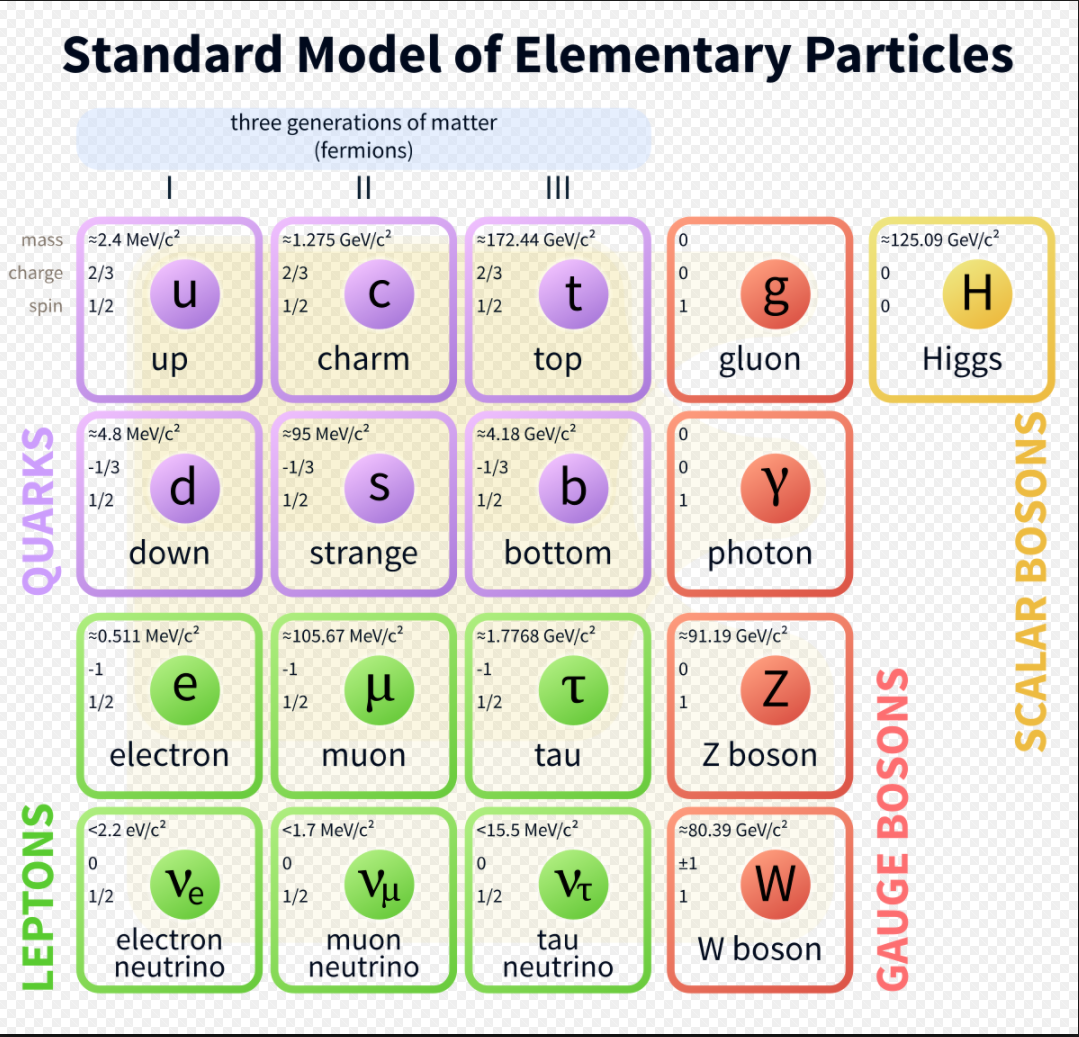
\includegraphics[width=\textwidth]{Elementary_particles_stdmodel}
    \newline
    \newline
    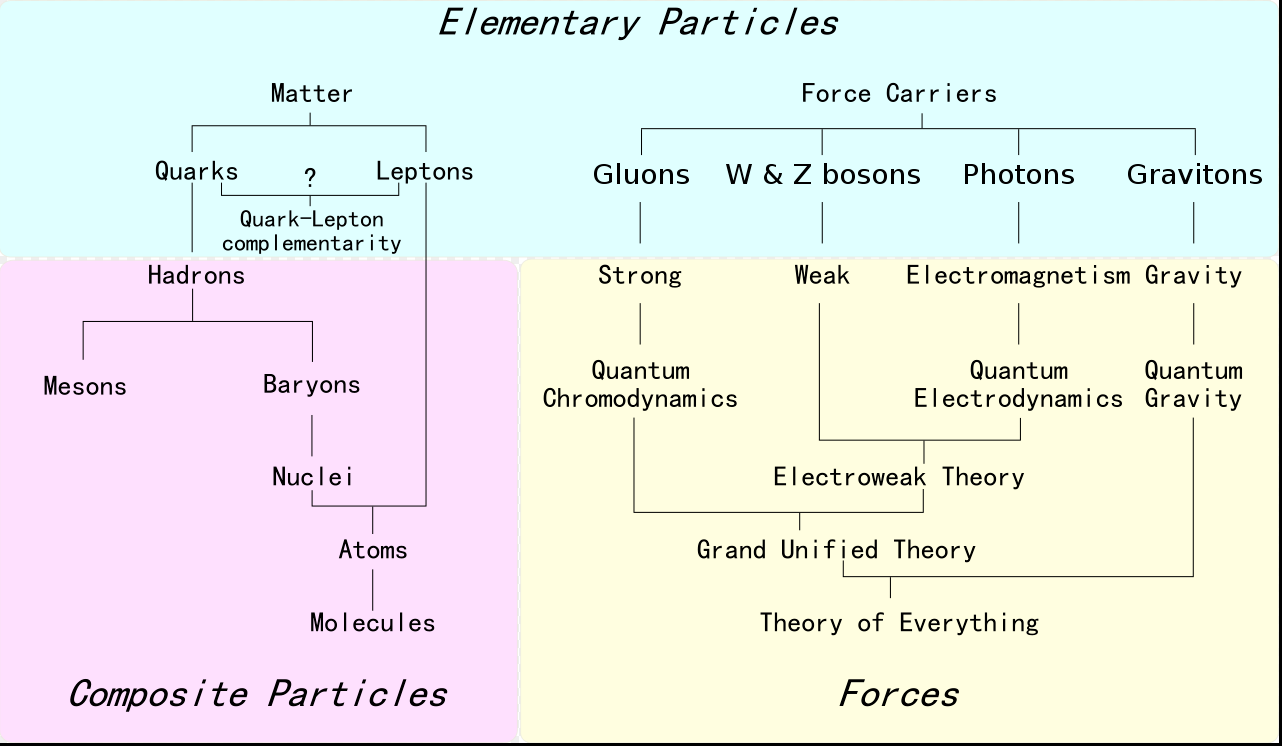
\includegraphics[width=\textwidth]{Elementary_particles_family}
    \newline
    \newline
    \newline
    \newline
    \textbf{nucleosynthesis} - the process that creates new atomic nuclei from pre-existing nucleons, primarily protons and neutrons.
    \newline
    \newline
    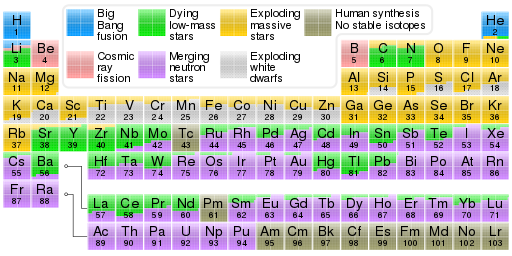
\includegraphics[width=\textwidth]{Nucleosynthesis_periodic_table}
    \newline
    \newline
    \newline
    \newline
    \textbf{big bang model of cosmology} - or hot big bang model - posits that the universe has expanded from an initially hot and dense to its current cooler state and that the expansion is still ongoing today.
    \newline
    \newline
    \textbf{planck blackbody} - or Bose-Einstein and the related Fermi-Dirac distributions.
    \newline
    \newline
    \textbf{Cosmic Microwave Background Radiation (CMBR)}
    \newline
    \newline
    \textbf{quintessence} - a hypothetical form of dark energy, more precisely a scalar field (with an equation of state), postulated as an explanation of the observation of an accelerating rate of expansion of the universe, rather than due to a true cosmological constant.
    \newline
    \newline
    \textbf{Friedmann-Robertson-Walker model} - simplfiying assumptions (homogeneous and isotropic) in Einstein's general relativity theory define the FRW family of cosmological models (solutions).
model
    \newline
    \newline
    \textbf{electromagnetic spectrum} - range of frequencies (the spectrum) of electromagnetic radiation and their respective wavelengths and photon energies.
    \newline
    \newline
    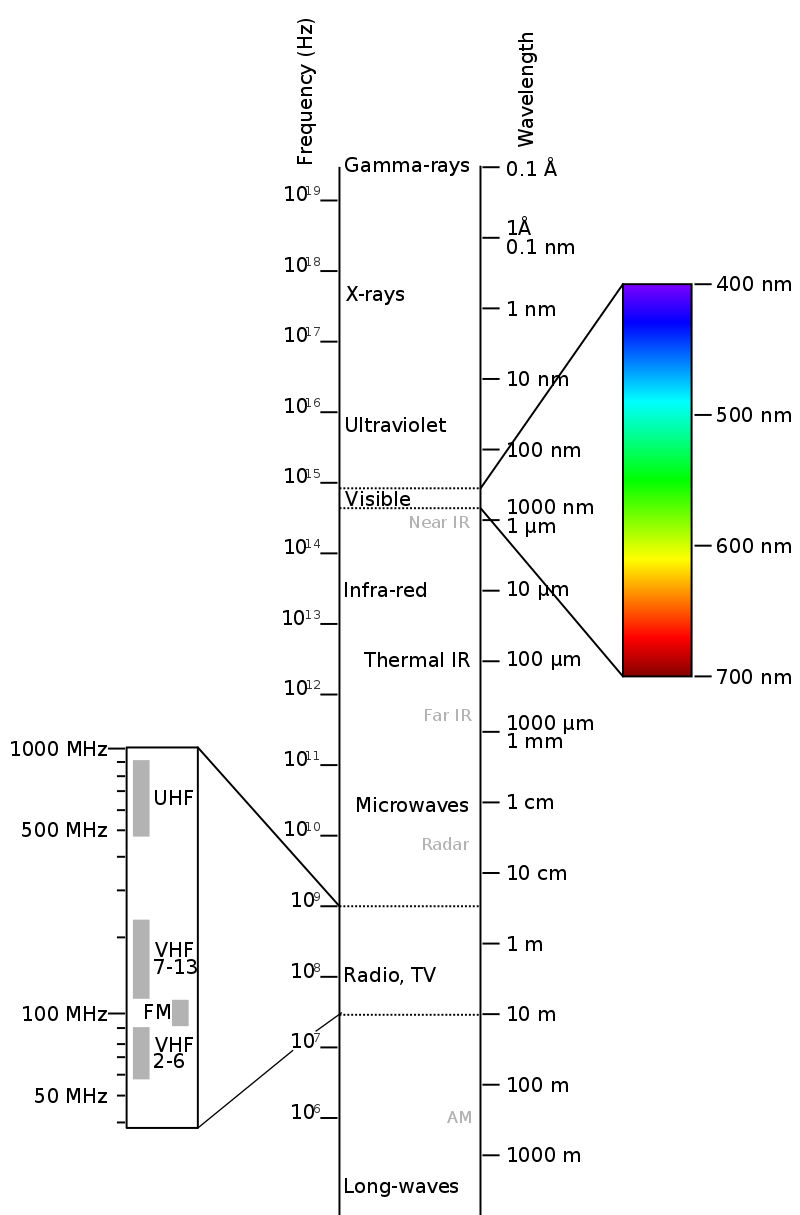
\includegraphics[width=\textwidth]{800px-Electromagnetic-Spectrum.png}
    \end{flushleft}



\pagebreak
\subsection{References List}\label{references}

      \cite{masksoftheuniverse}
      \cite{cosmology}
      \cite{beyondthegalaxy}
      \cite{cosmologyforthecurious}
      \cite{astrophysicsforpeopleinahurry}
      \cite{afortunateuniverse}
      \cite{abrieferhistoryoftime}
      \cite{thebigpicture}
      \cite{justsixnumbers}
      \cite{blackhole}
      \cite{thehiddenreality}
      \cite{thefabricofthecosmos}
      \cite{realativity}
      \cite{thegranddesign}
      \cite{thecopernicuscomplex}
      \cite{gravitysengines}
      \cite{auniversiefromnothing}
      \cite{projecttuva}
      \cite{einsteinemb}
      \cite{appec}
      \cite{gravity}
      \cite{introtocosmology}
      \cite{astrophysicsinanutshell}
      \cite{gravitysfatalattraction}
      \cite{blackholesandtimewarps}
      \cite{cosmologytoday}
      \cite{cosmologyabriefrefreshercourse}
      \cite{connectingquarkswiththecosmos}
      \cite{cosmologyaresearchbriefing}
      \cite{expositiononinflationarycosmology}
      \cite{amostincomprehensiblething}
      \cite{specialrelativity}
      \cite{thefirstthreeminutes}
      \cite{searchingforstarsonanislandinmaine}
%\maketitle

%    This document is an example of BibTeX using in bibliography management. Three items are cited: \textit{The \LaTeX\ Companion} book \cite{latexcompanion}, the Einstein journal paper \cite{einstein}, and the Donald Knuth's website \cite{knuthwebsite}. The \LaTeX\ related items are \cite{latexcompanion,knuthwebsite}.


\bibliographystyle{unsrt}%Used BibTeX style is unsrt
\bibliography{tentominusthirtyseconds}


\end{document}
